%!TEX root = ../report.tex
\documentclass[report.tex]{subfiles}
\begin{document}
    \chapter{Solution}
    We discussed various kind of controllers in chapter \ref{State of the Art} session \ref{Controller} and the background knowledge of Popov-Vereshchagin hybrid solver in chapter \ref{Background}.In this chapter The proposed robot archtechture session will present how the forementioned sovler and controller implement on the robot. Session extension of Robif2b will discuss how to modify Robif2b such that the communication between robot and the software interface can be extended.

    \section{Proposed robot archtechture}

    Figure \ref{fig:sys} shows the robot system archtechture majorly consist of a cascaded controller, the Popov-Vereshchagin solver and the robot. In \ref{Background} mentioed the inputs of the Popov-Vereshchagin solver. The cascaded controller composes of a P-position controller and a P-velocity controller. The main program fetch the instantaneous joint angle $q$ from the robot, then perform forward kinematic to compute the current Cartesian pose of the robot's end-effector $X_{curr}$. Then calculate the position error term $X_{err}$ by calling \textit{diff($X_{goal}$,$X_{curr}$)} mentioned in chapter \ref{diff_frame} where $X_{goal}$ is the desired pose of the robot's end-effector of the current task. The P-position controller compute the position control signal $ctrl\_sig_{pos}$ and feeds into P-velocity controller with the current Cartesian of the end-effector $\dot{X}_{curr}$. Before the main loop starts, $\dot{X}_{curr}$ is assumed to be zero in all linear and angular directions. After the first iteration, by calling function $getLinkCartesianPose()$ from vereshchagin solver, it will update the $\dot{X}_{curr}$. The error is the difference between position control signal $ctrl\_sig_{pos}$ and $\dot{X}_{curr}$. P-velocity controller computes the control signal , which directly being set as acceleration energy setpoints $\beta_N$ in the Popov-Vereshchagin solver.\\
    We mentioed the inputs of the Popov-Vereshchagin solver in \ref{Background} and from above ,joint angles and velocities $q$ and $\dot(q)$ of the end-effector at the current time frame can be obtained from the robot. Feedfoward joint torques remain zero since it is not necessary to propose task specification on joint torques such as spring and/or damper-based torques in robot's joints\cite{Vukcevic2020}. The external forces driver $F_{ext}$ will be set to a certain value according the task specification. In the experiement,$F_{ext}$ is set to some value to counter friction during contact situation. the details will be further explained in next chapter.
    As we discussed in \ref{Task interfaces}, the structure of $\alpha_N$ depends on the task specification. For example when the robot arm is moving in the mid-air, the direction of both linear and angular motion should be constrainted and in a contact situation, the constraint of linear z direction should be disabled. At last, $\beta_N$ is being controlled by the cascaded controller that is forementioned.

    The solver requires the robot chain during declaration. There are two ways to implement such robot chain. the first one is to create a robot chain class and using typical KDL robot declaration: \textit{chain.addSegment()} to create the chain by referring to the Kinova robot manual. However, KDL expresses the rigid-body inertia in the link's tip frame whereas the manual chooses the link's root frame. Hence, inverse transformation is needed. Unfortunately, the frame assignment for the DH parameters in the manual is also encountering the same issue, so additional transformations of the inertia would be required when referring to the DH parameters on user manual. To avoid such problem, we are using kdl\_parser library \cite{kdl_parser},\cite{roskdlparser}. KDL utilizes a tree structure to model and store the kinematic and dynamic characteristics of a robot mechanism. The kdl\_parser offers utilities to create a KDL tree based on an XML robot description in URDF format Originally, this was a ROS package. However, as our project is not developed within the ROS framework, we have removed the dependencies on ROS.

    The Popov-Vereshchagin solver has two properties: It does not support fixed joint and tree structure. So in kdl\_parser, we have to create the chain until bracelet link instead of the end-effector frame since the gripper has a tree structure. In order to construct the correct robot chain that includes the gripper, we have to add the weight of gripper in the bracelet link in the urdf file such that the weight of gripper is taking into the account when computing robot dynamics \cite{gripper}.
    \begin{figure}[h]
        \centering
        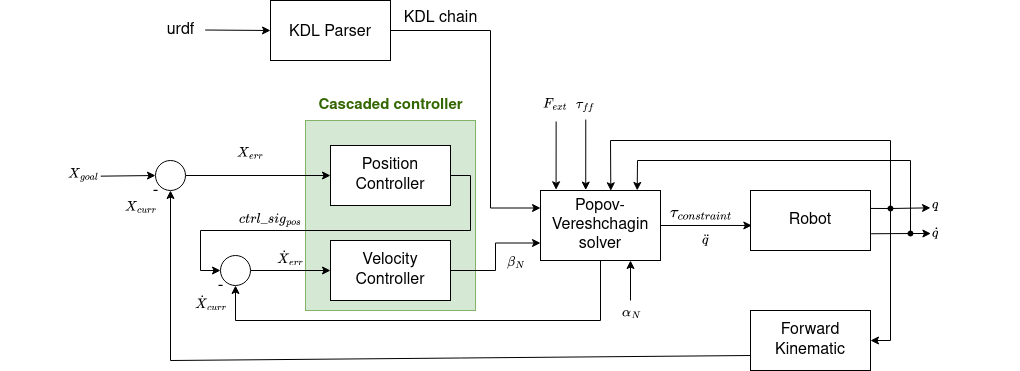
\includegraphics[width=1\linewidth]{images/system_arch.png}
        \caption{A generic control diagram illustrate the interactions of end-effector (task)
        pos and cascaded controllers with the constrained dynamics
        algorithm. It shows the connection between controller, solver and robot.}
        \label{fig:sys}
    \end{figure}

    \section{Extension of Robif2b}
    In this research and development project, the Kinova® Gen3 Ultra lightweight robot manipulator is employed, and a Kinova Kortex API client facilitates communication between the robot and the software\cite{Kinovaapi},\cite{KINOVA_userguide}. The script employs low-level servoing control as it circumvents the kinematic control library. This approach permits clients to independently control each actuator by transmitting command increments at a frequency of 1 kHz to increase the respond speed. Figure \ref{fig:kinova_low} show the conenction between actuator, robot base and client in Low-level servoing mode.\begin{figure}[h!]
        \centering
        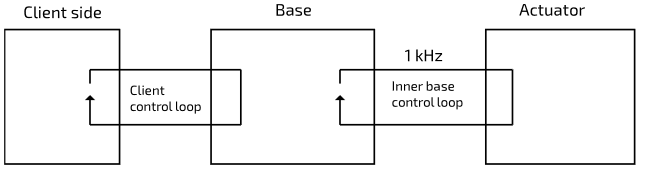
\includegraphics[width=1\linewidth]{images/kinovalowlevel.png}
        \caption{Conenction between actuator,robot base and client in Low-level servoing}
        \label{fig:kinova_low}
    \end{figure}
    If we control robot with the Kortex api directly, we need to establish TCP/UDP connection and create session for data connection. Beside this complex implementation, there is another simple alternative. Robif2b is robot control interface wraps the session creation, connection establishment and communication between actuator, base and client side\cite{Rosym-Project}. In the original Robif2b, the connection of actuator is already being establish to received the feedback from the base such that we can write a single line of command to receive the current status of base and actuators. Nonetheless, it didn't encompass the capability to retrieve the voltage and current status of the gripper actuator. The code snippet below demonstrates how the port is configured to receive current status updates for the base and actuators:
    \begin{lstlisting}[caption = {Struct of the enabled ports for base and actuator of Kinova kortex api in Robif2b},label={lst:Robif2b}]
    struct robif2b_kinova_gen3_nbx
    {
        // Configuration
        struct robif2b_kinova_gen3_config conf;
        // Ports
        const double *cycle_time;               // [s]
        enum robif2b_ctrl_mode *ctrl_mode;
        double *jnt_pos_msr;                    // [rad]
        double *jnt_vel_msr;                    // [rad/s]
        double *jnt_trq_msr;                    // [Nm]
        double *act_cur_msr;                    // [A]
        double *act_vol_msr;                    // [V]
        double *gripper_pos_msr;
        const double *jnt_pos_cmd;              // [rad]
        const double *jnt_vel_cmd;              // [rad/s]
        const double *jnt_trq_cmd;              // [Nm]
        const double *act_cur_cmd;              // [A]

        const double *gripper_pos_cmd;  
        double *imu_ang_vel_msr;                // XYZ [rad/s]
        double *imu_lin_acc_msr;                // XYZ [m/s^2]
        
        bool *success;
        // Internal state
        struct robif2b_kinova_gen3_comm *comm;
        enum robif2b_ctrl_mode ctrl_mode_prev;
    };
\end{lstlisting}
Line 12,13 and 19 are the extended port from original Robif2b such that we can retrieve the current voltage of each joint and the gripper position and we able to send the command to the gripper via sending the gripper position (0-100) with \textit{gripper\_pos\_cmd}. We can extend this struct according to the kortex api manual \cite{Kinovaapi} according to the need of evaluation.
Before sending the command to gripper to receive its current state or control the gripper, we have to declare the connection to the base and gripper. The code segment below is the extended code of gripper connection.
\begin{lstlisting}[caption = {Establish connection between base and gripper},label={lst:Robif2b_gripper}]
    // Initialize interconnect command to current gripper position.
    comm->command.mutable_interconnect()->mutable_command_id()->set_identifier(0);
    comm->gripper_command = comm->command.mutable_interconnect()
        ->mutable_gripper_command()->add_motor_cmd();
\end{lstlisting}

In function \textit{robif2b\_kinova\_gen3\_update(struct robif2b\_kinova\_gen3\_nbx *b)} , we can add the following line to control the gripper by simply passing the gripper position to \textit{gripper\_pos\_cmd} 


\end{document}
